\chapter{基于噪声标签的语义分割}
% 在这个工作中,我们为图像语义分割提出了一种新的鲁棒的学习策略,目标是利用图像的结构先验和像素标签的相关性。为此,我们采用了图像的超像素表示,并设计了一个迭代学习方案,这个方案结合了分割网络的噪声感知训练过程和噪声标签改进过程,两者都由超像素引导。这种结合使我们能够更好地利用分割标签的结构约束来进行模型学习,从而有效地减轻噪声标签的影响。我们注意到,虽然超像素在最近的工作中也被采用\citep{li2019supervised},但他们只用来改进噪声标签,而忽略了训练期间噪声标签的影响。

真实世界中,完全准确的图像标签是很少的,由于标注图像、标注者、标注环境等多种因素,噪声标签难以避免。
本章中我们研究基于基于噪声标签的语义分割,这是弱监督语义分割的一个方向。为了充分利用标签中的有效信息而避免其中的噪声干扰,我们提出采用协同教学的模型框架,并随后设计了一个鲁棒的迭代学习策略。我们的方法利用了图像与标签的结构先验约束,并且结合了有噪声感知的训练过程和噪声标签改进过程。这种模型与学习策略的结合,有助于我们充分挖掘标签信息来实现高性能分割。

本章分为以下四个部分。在第一节描述基于噪声标签的语义分割任务,第二节详细介绍我们的模型与训练方法,包括超像素表示、迭代学习策略的网络更新方法、训练停止标准和标签更新方法等。
第三节为实验部分,包括实验数据集、实现细节、对比结果、消融实验等部分。最后是本章小节。

\section{问题概述}
与通常的语义分割任务不同的是,基于噪声标签的分割任务中,训练图像的标签有一部分是错误的。这些标签噪声会误导网络的正常训练,从而影响最终的分割性能。
形式化地,给定一张图像 $\mb{X}$,其对应的噪声标签 $\mb{Y}=\{Y_i\}_{i=1}^M$,其中 $Y_i\in\{1,\cdots, C\}$,$C$ 是语义类别的数目,$M$ 是图像像素的数目。
我们的目标是充分利用$\mb{Y}$中的正确信息来训练分割模型。

为此,我们提出了一种语义分割的稳健学习策略,其目的是利用图像标签掩膜中的结构约束,并充分利用可靠的像素标签进行有效的学习。实现上,我们采用了基于超像素的数据表示方法,并设计了一种迭代学习方法,联合地优化网络参数和改进噪声标签。

\section{方法}
我们的模型及训练方法如图~\ref{fig:nss_overview}所示,我们使用两个并行的分割网络来进行协同教学,以避免单个网络的过拟合或不稳定学习。训练中,它以超像素表示作为指导,在迭代学习过程中联合地更新网络参数并改进噪声标签。每轮迭代会先选择小损失值(标签置信度高)的超像素来同时更新两个网络,达到停止标准后,根据网络预测结果来改进一部分超像素的标签。

具体来说,给定分割网络框架和有噪声的训练数据,我们首先计算生成输入图像的超像素。基于这样的像素聚合分组,我们的迭代学习过程在有噪声感知的网络训练阶段和标签改进阶段之间交替进行,直到不再有增益效果。对网络更新阶段,我们采用多视图学习框架,联合训练分割网络的两个实例。对于标签改进阶段,我们使用两个训练好的网络的输出来估计超像素标签的可靠性,并更新不可靠的标签。下面我们首先在~\ref{sec:p2_1}节介绍我们的超级像素化程序,然后在~\ref{sec:p2_2}节介绍迭代学习的两个阶段。

    \begin{figure*}[tbp]
        \centering 
        \includegraphics[width=1.0\textwidth]{img/c4/model_overview2.pdf}
        \bicaption{我们的鲁棒学习方法。分割模型以超像素表示作为指导,在迭代学习过程中联合地更新网络参数并改进噪声标签。每轮迭代会先选择小损失值(标签置信度高)的超像素来同时更新两个网络,达到停止标准后,根据网络预测结果来改进一部分超像素的标签。}
        {Overview of our robust training process. We use superpixels as our guidance in an iterative learning process which jointly updates network parameters and refines noisy labels. Each iteration selects superpixels with small losses to update two networks and relabels a set of superpixels based on network outputs.} %In inference mode, we use well-trained networks to predict the segmentation map.
        \label{fig:nss_overview}
    \end{figure*}


\subsection{超像素表示} \label{sec:p2_1}

为了在分割方法中利用图像的结构先验和像素标签的空间相关性,我们首先为训练图像计算生成对应的超像素表示。在之前的一些工作中,这种超像素表示已被证明对不同的医学图像模态是有效的,例如\citet{qin2018superpixel}对 CT,\citet{tian2015superpixel}对 MR 和\citet{daoud2019automatic}对 US 图像。
具体地,我们使用现有的超像素化方法 SLIC\citep{Achanta2012SLICSC},将每个图像划分为一组同质区域的集合。对于彩色图像,我们采用 CIE-lab 颜色空间来表示像素特征,而对于其他模态,如 X 射线图像,我们同时使用像素强度和用噪声感知方法(比如~\citet{Wei2020CombatingNL})训练的 U-net 的深层特征。\footnote{在胸部 X 射线数据集上~\cite{Shiraishi2000DevelopmentOA,Ginneken2006SegmentationOA},我们的超像素在每个图像800个超像素的设置下取得了低于 0.32 的下分割误差(undersegmentation errors),这与自然图像可比的数值\citep{Achanta2012SLICSC}。}

我们假设每个超像素中的像素有相近的真实标签,这使我们能够施加标签掩膜的结构约束,并且更好地保留物体的边缘。更重要的是,在随后的鲁棒网络学习和标签改进中,我们把超像素视为一个数据样本的基本单元。这使我们能够通过汇聚每个超像素的像素信息,以更可靠的方式来估计像素标签的噪声水平。

\subsection{迭代学习} \label{sec:p2_2}
我们提出了基于超像素表示的迭代学习策略,其目的是充分利用干净的像素标签,同时减少噪声标签的影响。我们为模型训练引入了一个迭代优化过程,每个迭代包括两个阶段:第一个阶段是有噪声感知的网络学习阶段,选择干净标签更新网络参数;第二个阶段是标签改进阶段,使用网络预测来纠正不可靠的标签。

\subsubsection{网络更新}

在第一阶段,我们通过将超像素表示纳入多视图学习框架来进行有噪声感知的网络学习。具体地,沿用协同教学策略~\citep{ren2018learning, jiang2018mentornet, Han2018CoteachingRT},我们选择具有小损失值\citep{arpit2017closer}的部分训练数据,来同时训练目标分割网络的两个实例。
小损失值一般代表着较高的标签可信度,作为区分干净标签与噪声标签的一个依据。而两个分割网络的同时训练,有助于实现两个网络互相约束和协同训练。
为了更好地选择具有干净标签的数据样本,我们设计了一个超像素级的损失函数,它结合了两个网络各自的超像素上的损失值和一致性约束\citep{Wei2020CombatingNL}。由于超像素中编码的结构先验,我们的损失函数为样本选择提供了可靠的引导。

形式上,给定一个图像 $\mb{X}$ 及其对应的噪声标签 $\mb{Y}$,我们生成图像对应的超像素图 $\mb{S} =\{S_i\}_{i=1}^M$,其中 $S_i\in\{1,2,\cdots, K\}$,$K$ 是超像素的数目。这里,$S_j=k$ 意味着像素 $j$ 属于超像素 $k$。

我们的目标是训练两个深度神经网络,分别用 $f(\cdot, \theta_1)$ 和 $f(\cdot, \theta_2)$ 表示。为了定义每个图像的损失,我们从两个网络生成预测概率图,表示为 $\mb{P}_s^i\in\mathbb{R}^{C \times K}, i=1,2$。然后我们通过每个超像素取平均,计算图像的超像素级的概率图 $\mb{P}_s^i\in\mathbb{R}^{C \times K}, i=1,2$ 以及相应的软标签 ${\mb{Y}_s}\in[0,1]^{C\times K}$:
\begin{align} \label{eq:joint_prob}
    \mb{P}^i_s(c,k) = \frac{1}{N(k)}\sum_{j:S_j = k} \mb{P}^i(c,j)
\end{align}
\begin{align}
    \mb{Y}_s(c,k) =\frac{1}{N(k)} \sum_{j:S_j = k}\mathds{1}(Y_j = c)
\end{align}
其中 $N(k) = |\{j:S_j = k\}|$ 是超像素的大小。受\citet{Wei2020CombatingNL}的启发,我们通过在每个超像素上结合分类损失和预测一致性损失,来定义超像素级的损失函数 $\ell^{sp}$:
\begin{equation}\label{l_k}
	\ell^{sp} = (1-\lambda)*(\ell_{ce}(\mb{P}^1_s,\mb{Y}_s) + \ell_{ce}(\mb{P}^2_s,\mb{Y}_s)) + \lambda *\ell_{kl}(\mb{P}^1_s,\mb{P}^2_s)
\end{equation}
其中 $\ell_{ce}$ 是预测对软标签的交叉熵损失,$\ell_{kl}$ 是对称的相对熵(Kullback-Leibler Divergence), $\lambda$ 是一个平衡因子。
第一项两个网络的分类损失,使得我们能优先选择小损失值(根据网络的记忆效应,其标签置信度高)的标签。第二项的预测一致性损失,则是为了挖掘较难的样本来训练。这些较难的样本可能本身不容易学习,导致损失值较大,但两个网络相似的预测可以增加其标签置信度,使得它们也加入训练提高性能。
通过在小损失标准中同时考虑以上两项,我们的目标是选择标签噪声低的训练数据进行选择,来更新模型参数,同时使两个网络的一致性最大化。

被选择的用于训练的像素比例标记为 $R$,我们通过小损失选择标准,选出一个超像素集 $\mathcal{\hat{D}}_s$,如下:
\begin{equation}
	{\mathcal{\hat{D}}}_s = {\arg\min}_{{\mathcal{D}_s}: N({\mathcal{D}_s})\ge R\cdot M} \sum_{k\in{\mathcal{D}_s}}\ell^{sp}_k 
\end{equation}
其中 $N({\mathcal{D}_s}) = \sum_{k\in {\mathcal{D}_s}} N(k)$ 是超像素集的总像素数目。
小损失选择过程后,我们根据平均损失来训练网络:
\begin{equation}
	\mathcal{L} = \frac{1}{N(\mathcal{\hat{D}}_s)}\sum_{S_i \in \mathcal{\hat{D}}_s}\ell_i
\end{equation}
其中 $\ell$ 的形式与公式~\ref{l_k} 一致,除了它定义在像素层面上。这里我们为了实现更有效的反向传播,跳过了公式~\ref{eq:joint_prob} 中的超像素级汇聚。

图~\ref{fig:vis_select} 给出了网络更新中选择过程的可视化。对比基于像素和基于超像素的选择结果,可以看出:我们的方法充分利用了图像的结构先验和空间关系,能在物体边缘选出更多信息量大的区域,选择的边缘也更准确,与理想的选择区域接近。

    \begin{figure*}[tbp]
        \centering 
        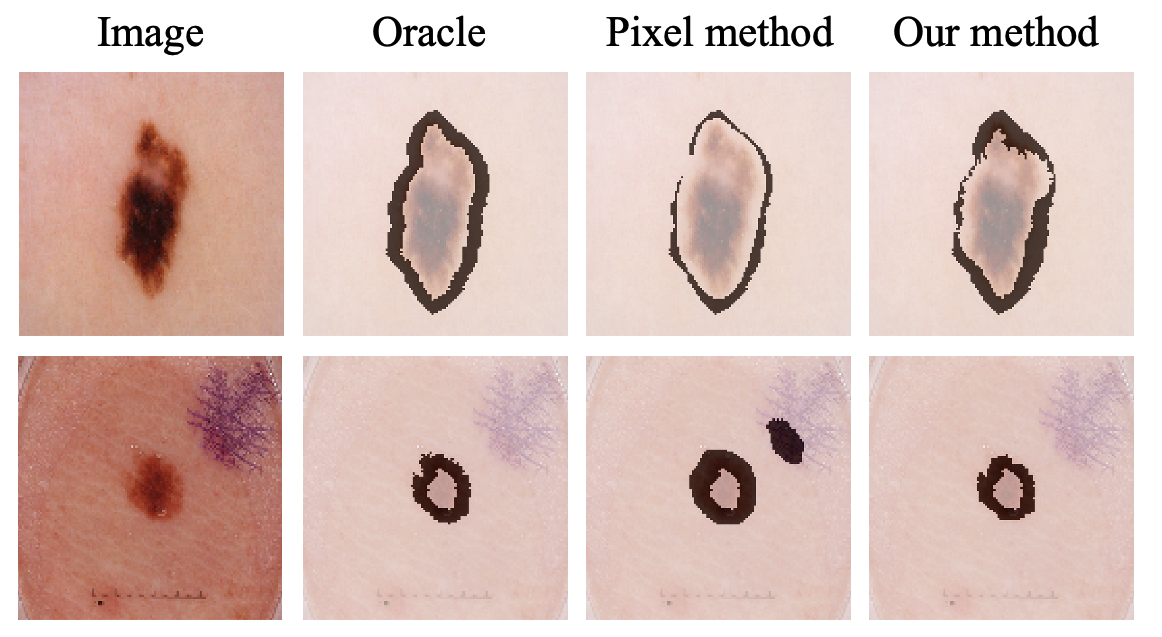
\includegraphics[width=1.0\textwidth]{img/c4/b_select2.png}
        \bicaption{网络更新中的选择过程的可视化结果。我们比较了基于超像素的方法与基于像素的方法。Oracle 对应理想的选择区域。浅色掩膜表示选择的区域,深色掩膜表示筛除的区域。}
        {Visualization results of our selection method in network updating. We compare our superpixel-based method with pixel-based method. Oracle is short for oracle selection map. We denote selected region in light matte, leaving sieved region in dark matte. }
        % (b) Red curves shows the groundtruth label, and blue curves shows the noisy or refined label.
        \label{fig:vis_select}
    \end{figure*}

\subsubsection{训练停止标准}
虽然前述的选择更新策略可以使网络利用大部分干净的标签数据来训练,但一些噪声标签仍会不可避免地被选中并逐渐影响模型的性能。为了解决这个问题,我们提出了一个标准,它在过拟合之前停止网络训练。我们的训练停止标准是根据所选数据和剩余数据之间的损失差距 $G_l$ 来定义的,如下:
\begin{equation}\label{loss_gap}
	G_{l} =    \frac{1}{K-|\mathcal{\hat{D}}_s|}\sum_{k \notin \mathcal{\hat{D}}_s}\ell_k^{sp} - \frac{1}{|\mathcal{\hat{D}}_s|}\sum_{k \in \mathcal{\hat{D}}_s}\ell_k^{sp} 
\end{equation}

直观地,深度模型倾向于首先学习干净数据中相对简单的模式,然后开始对标签噪声进行过拟合\citep{arpit2017closer}。因此,$G_{l}$ 首先逐渐升高,然后开始降低。基于这一观察,我们在 $G_{l}$ 达到最大值时开始下降之前停止模型训练。
训练结束后,实验观察到两个对等网络的输出非常相似。因此,在测试/部署阶段我们任意选择一个网络进行预测。

\subsubsection{标签更新}

在标签更新阶段,我们使用训练好的网络来估计超像素标签的可靠性,并对不可靠的超像素子集更新标签。具体来说,我们选择出具有大损失值的超像素,这表明模型预测和它们的标签之间存在明显的不一致。然后,我们根据预测的类别标签对选择的部分进行重新标注。形式上,我们根据超像素的损失来定义不可靠的超像素 $\mathcal{\hat{D}}_u$,并计算出预测的超像素标签 $\mb{\hat{Y}} =\{\hat{Y}_i\}_{i=1}^K,\hat{Y}_i\in \{1,\cdots,C\}$,如下:
\begin{align}
    {\mathcal{\hat{D}}}_u &= {\arg\max}_{{\mathcal{D}_u}: N({\mathcal{D}_u})\le (1-{R})\cdot M} \sum_{k\in{\mathcal{D}_u}}\ell_k^{sp} \\
    \hat{Y}_k &= \mathop{\arg\max}_{c}\frac{1}{2}(\mathbf{P}_s^1(c,k) + \mathbf{P}_s^2(c,k))
\end{align}
其中 $\ell_k^{sp}$ 在公式~\ref{l_k}中定义,$R$ 是之前提到的选择比例。最后,我们更新像素级标签图 $\mb{Y}'=\{Y'_i\}_{i=1}^M, Y'_i\in\{1,\cdots, C\}$ 为
\begin{equation}
	Y_i' = \mathds{1}(S_i \in {\mathcal{\hat{D}}}_u )\hat{Y}_{S_i} + \mathds{1}(S_i \notin {\mathcal{\hat{D}}}_u )Y_i
\end{equation}
在标签更新之后,我们用 $\mb{Y}'$ 替换 $\mb{Y}$,用一个固定的比例 $\gamma$ 增加 $R$ ,然后开始下一轮迭代。

我们对比了基于像素和基于超像素的标签更新结果,如图~\ref{fig:vis_correct} 所示。红色曲线内的区域为真实标签,蓝色曲线内的区域为噪声标签(第二列)或更新后的标签(第三、四列)。可以得出,我们的方法结果更接近真实标签,在物体的边缘区域的效果提升很多。
    \begin{figure*}[tbp]
        \centering 
        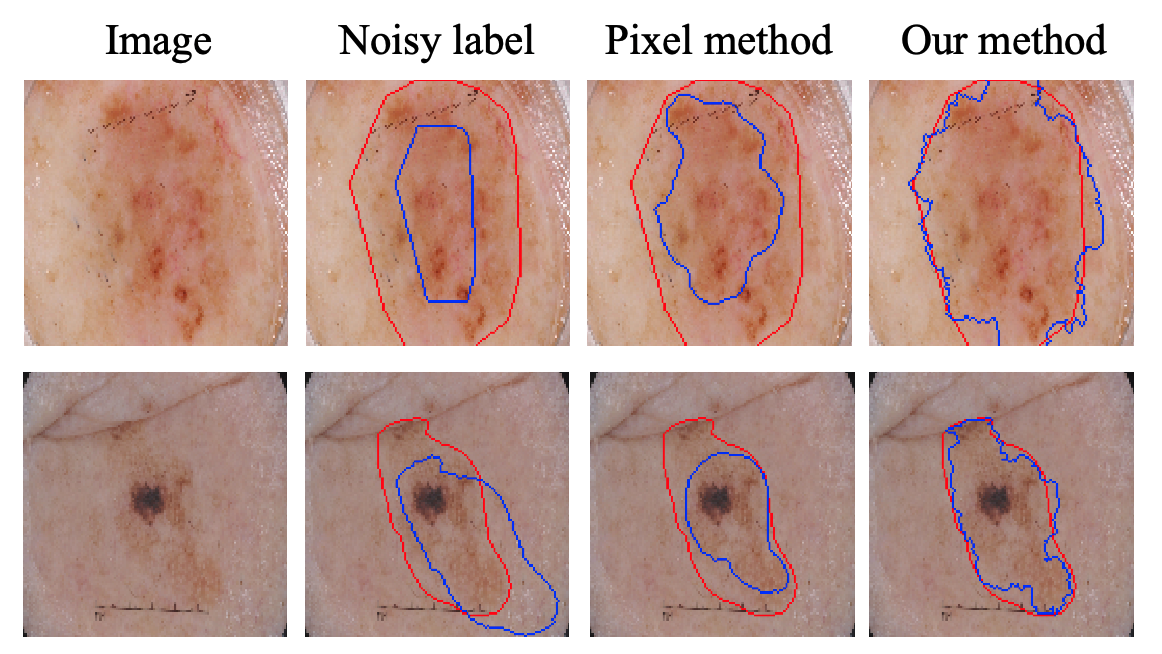
\includegraphics[width=1.0\textwidth]{img/c4/b_correct2.png}
        \bicaption{标签更新过程的可视化结果。前两列分别是原始图像和噪声标签,我们在后两列比较了基于像素和基于超像素的更新结果。红色曲线内的区域为真实标签,蓝色曲线内的区域为噪声标签或更新后的标签。}
        {Visualization results of our label refinement. The first two rows show original images and noisy labels, respectively, and we compare refined labels based on pixel-level and superpixel-level methods in the last two rows. Red curves shows the groundtruth label, and blue curves shows the noisy or refined label.}
        \label{fig:vis_correct}
    \end{figure*}

\section{实验}


\subsection{实验数据集}




\subsection{实验设置}




\subsection{ISIC 数据集}




\subsection{消融实验}




\subsection{JSRT 数据集}




\section{本章小节}
